\section{Backend}
\author{Stefano Pyringer}

\subsubsection{Erstellung der Datenbank}
Für die Erstellung der Datenbank wurde der Modellierungsansatz Code-First angewendet. 
Das Mapping der EF Core Datenbank ist in der Klasse FeedbackDbContext.cs definiert. Die Tabellen entsprechen der in Kapitel 2 Abbildung 3 
abgebildeten ERD.

\begin{figure}[h]
    \begin{center}
        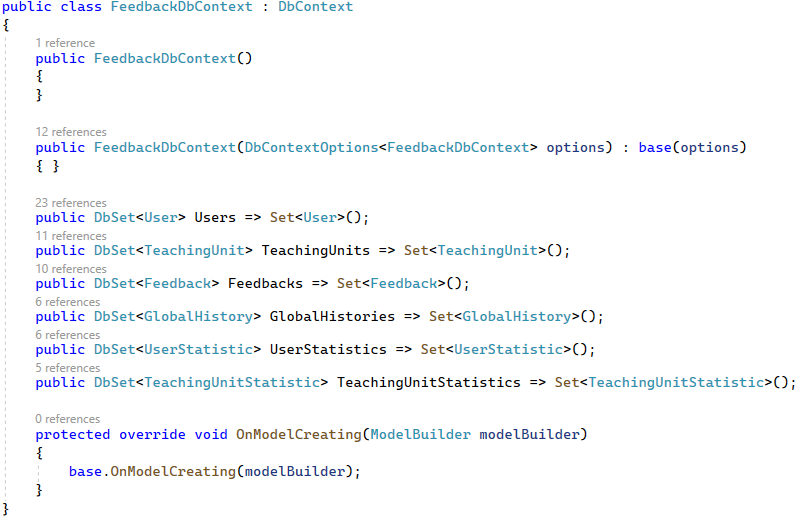
\includegraphics[width=15cm]{./pics/Persistance/FeedbackDbContext.png}
    \caption[FeedbackDbContext]{FeedbackDbContext.cs Mappping}
    \end{center}
\end{figure}

Die Tabellen wurde 
mit Klassen erstellt, die mit Annotationen ausgezeichnet wurden. Sie sind im Core Bereich der Solution unter Models zu finden.
Eine Besonderheit ist die Model-Klasse TeachingUnit in diesem Projekt, da sie die Möglichkeit mithilfe eines bool-Atributes bietet, 
ob eine Lehreinheit öffentlich sichtbar ist.

\begin{figure}[h]
    \begin{center}
        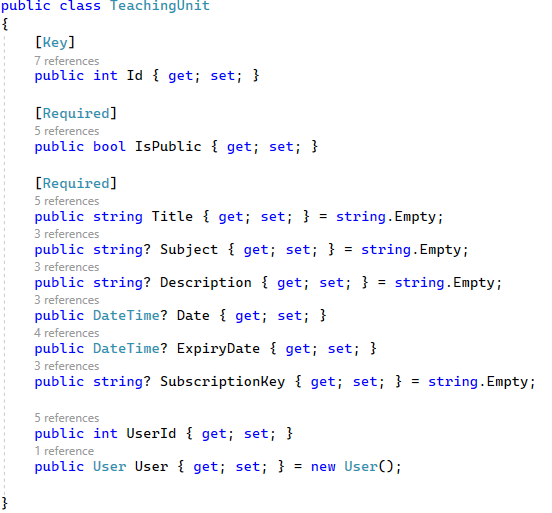
\includegraphics[width=12cm]{./pics/Persistance/TeachingUnitModelEfCore.png}
    \caption[TeachingUnitModel]{Model-Klasse TeachingUnit.cs}
    \end{center}
\end{figure}

Beide Datenbanken für Feedback und Identity an sich wird lokal in Microsoft SQL Server erstellt und initialisiert. 
Die Connection Strings sind in appsettings.json definiert.

\newpage
\subsection{Datenbank (Persistance)}
\author{Stefano Pyringer}
Die Controller der Web API greifen auf die Daten im Persistance-Teil der Anwendung zu. Es existieren 3 Repositories 
die den Datenzugriff der Feedback API im Hintergrund ermöglichen. Alle Methoden der Repositories sind asynchron und 
ermöglichen somit das Multitasking von Requests. Für die Datenzugriffe in den Methoden wurde LINQ verwendet.

\begin{figure}[h]
    \begin{center}
        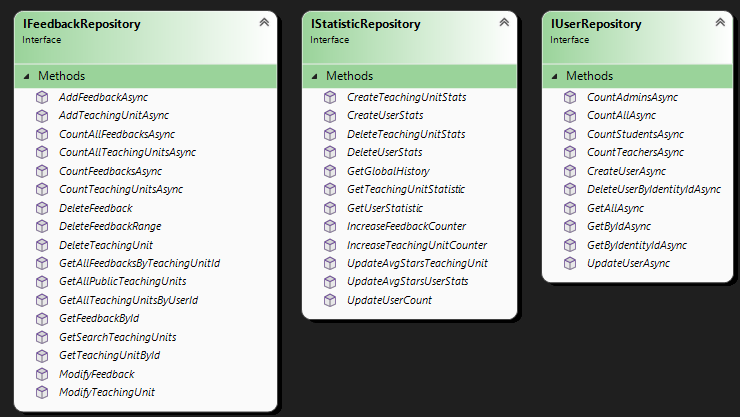
\includegraphics[width=15cm]{./pics/overview-repo-interfaces.png}
    \caption[overview Repos]{Überblick der Methoden der Repositories}
    \end{center}
\end{figure}

\subsubsection{User-Repository}
\author{Stefano Pyringer}
Dieses Repository stellt Datenzugriffsmethoden für die Benutzerkontoverwaltung bereit. Mit diesen Methoden 
werden User abgefragt, erstellt, geändert und gelöscht. Zusätzlich stellt es Zählmethoden für Statistiken bereit.

\subsubsection{Statistic-Repository}
\author{Stefano Pyringer}
Diese Methoden stellen Methoden für die Statistik der Anwendung bereit. Wenn ein Benutzer erstellt oder gelöscht wird, 
so muss auch die verknüpfte User-Statistik-Tabelle erstellt oder gelöscht werden. Die Umsetzung ist in der folgenden Abbildung sichtbar.

\begin{figure}[h]
    \begin{center}
        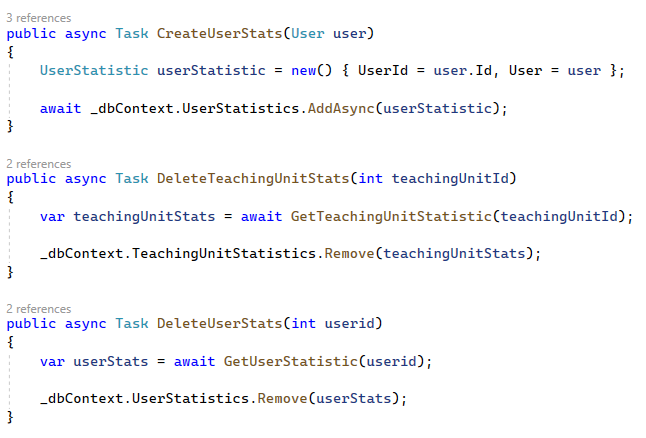
\includegraphics[width=15cm]{./pics/Persistance/UserStats.png}
    \caption[Userstats]{StatistikRepository Methoden Create/Delete}
    \end{center}
\end{figure}

\subsubsection{Feedback-Repository}
Sie ist das Herzstück der Persistance-Schicht des Projektes. In diesem Repository werden die Lehreinheiten und Feedbacks 
verwaltet. Wie beim Statistik Repository müssen auch im Falle einer Löschung einer TeachingUnit alle dazugehörigen Feedbacks gelöscht werden.

\begin{figure}[h]
    \begin{center}
        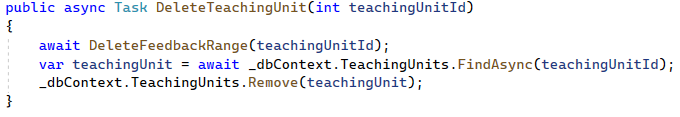
\includegraphics[width=15cm]{./pics/Persistance/DeleteTeachingUnit.png}
    \caption[DelTeachingUnit]{Methode für Löschung einer TeachingUnit}
    \end{center}
\end{figure}

\newpage
\subsection{Web API}
\author{Stefano Pyringer}

\subsubsection{Benutzerverwaltung}
\author{Stefano Pyringer}

\begin{figure}[h]
    \includegraphics*[width=15cm]{./pics/Screenshot_Swagger_Auth.png}
    \caption[Swagger Benutzerverwaltung]{Screenshot Swagger Web API Dokumentation Benutzerverwaltung}
\end{figure}

Für das Usermanagement wird das NuGet Package ASP NET Identity verwendet. Der Authenticate-Controller ermöglicht die Registrierung, den Login und die Löschung des Benutzerkontos. 
Zusätzlich kann das Passwort und die E-Mail Adresse nachträglich geändert werden. Schüler und Lehrende werden durch Rollen getrennt.
Bei erfolgreicher Authentifizierung wird ein gültiger JSON Web Token zurückgesendet. 

Der Benutzername muss folgende Kriterien erfüllen:
\begin{itemize}
    \item mindestens 6 Zeichen
    \item maximal 26 Zeichen
    \item keine Leerzeichen
    \item keine Sonderzeichen (Umlaute sind erlaubt)
\end{itemize}

Das Passwort hat folgende Mindestanforderungen:
\begin{itemize}
    \item mindestens 6 Zeichen
    \item keine Leerzeichen
    \item mindestens einen Großbuchstaben, einen Kleinbuchstaben und eine Zahl
\end{itemize}

Diese Anforderungen sind in der Start-Up Konfiguration der ASP NET Core Web API festgelegt und werden zusätzlich von 
der Klasse AuthenticateValidations.cs kontrolliert. Im Fehlerfall wird ein entsprechender HTTP-Fehlercode zurückgegeben.

Der UserAccount-Controller ermöglicht das Hinzufügen folgender Daten:
\begin{itemize}
    \item Titel
    \item Vorname
    \item Nachname
    \item Geburtsdatum
    \item Lehranstalt
\end{itemize}

\begin{figure}[h]
    \includegraphics*[width=15cm]{./pics/screenshot_Startup_PwUserReq.png}
    \caption[PW User Requirements Startup]{Screenshot Startup.cs Benutzername und Passwort Anforderungen}
\end{figure}

\newpage
\subsubsection{Authentifizierung}
\author{Stefano Pyringer}
Die Login-Methode sendet ein HTTP OK Response mit dem gültigen JWT Token als Objekt zurück. 
Der Token ist 15 Minuten lang gültig und beinhaltet die Id des Benutzerkontos und deren Rolle. 
Dieser erlaubt es, je nach Rolle, Zugriff auf die geschützten Bereiche der Web API.

\begin{figure}[!h]
    \includegraphics*[width=15cm]{./pics/screenshot_jwt_create.png}
    \caption[JWT create]{Screenshot JWT Token Erstellung detailliert}
\end{figure}

\newpage
\section{Frontend}
\author{Mirzet Sakonjic}
\subsection{Login}
Die Anwendungsseite wird ausschließlich in der Oberfläche realisiert, 
indem das Bild in einem separaten Ressourcenordner gespeichert und mit <img> 
angezeigt wird. Das Bild auf der Startseite ist urheberrechtlich geschützt, 
da sich dieses eine Bild nur auf der Anmeldeseite befindet. Beim Einloggen gibt 
der Nutzer seine E-Mail-Adresse und sein Passwort ein, die bereits ausgelesen 
und im Hintergrund in der Datenbank gespeichert wurden. Bei Bedarf kann ein 
neuer Benutzer angelegt werden. Die Validierung überprüft, ob die E-Mail-Adresse 
und das Passwort eingegeben wurden. Es überprüft auch Passwortregeln wie Länge, 
Großbuchstaben oder zusätzliche Zeichen.
\begin{figure}[h]
    \begin{center}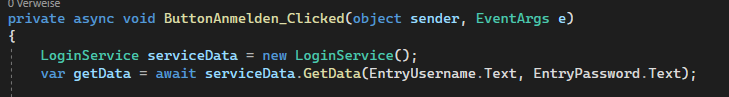
\includegraphics[width=10cm]{pics/Xamarin Frontend/1.png}
    \caption[Login]{Button Login}
    \end{center}
\end{figure}
\newline
Wenn der User auf den Button „Login“ drückt, wird ein LoginService-Request mit der
eingegebenen E-Mail und Passwort ans Backend gesendet. Wenn die Zugangsdaten
stimmen und der User vorhanden ist, werden die Logindaten inklusive Username
zurückgesendet und in der globalen Komponente abgespeichert, damit im gesamten
Projekt darauf zugegriffen werden kann.
\begin{figure}[h]
    \begin{center}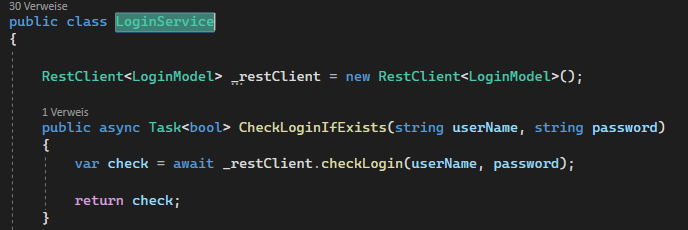
\includegraphics[width=10cm]{pics/Xamarin Frontend/2.png}
    \caption[Login]{RestClient}
    \end{center}
\end{figure}
\newline
\newpage
Mit Hilfe von RestClient erstellen wir ein LoginModel und fügen es in eine bool-Variable ein, um zu antworten, ob die Anmeldung erfolgreich war oder nicht, d.h. ob das Profil existiert oder nicht.
\begin{figure}[h]
    \begin{center}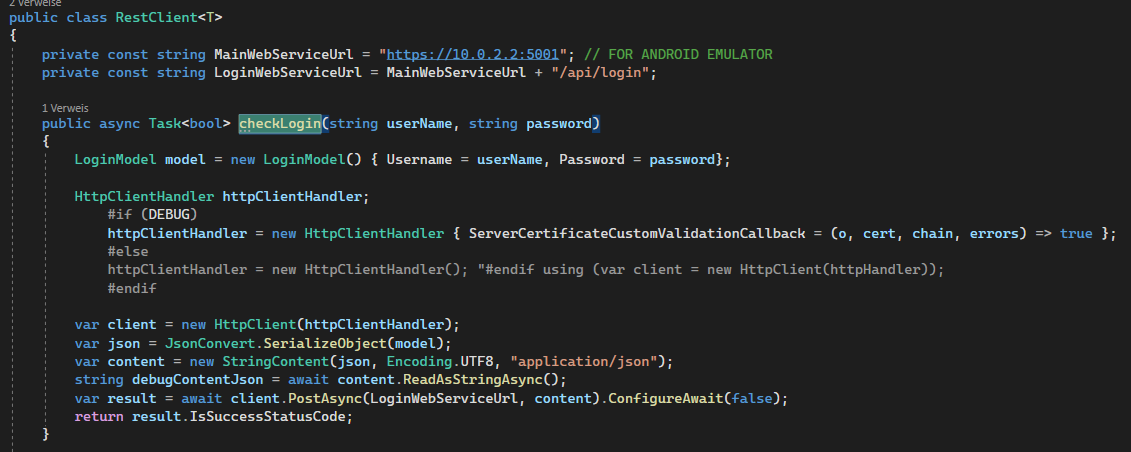
\includegraphics[width=10cm]{pics/Xamarin Frontend/3.png}
    \caption[Login]{HttpClient}
    \end{center}
\end{figure}
\newline
Sollten die Zugangsdaten nicht stimmen, wird eine Fehlermeldung angezeigt.
Nach dem erfolgreichen Laden aller Daten wird der User zu der Startseite
weitergeleitet.
\newline
\begin{figure}[h]
    \begin{center}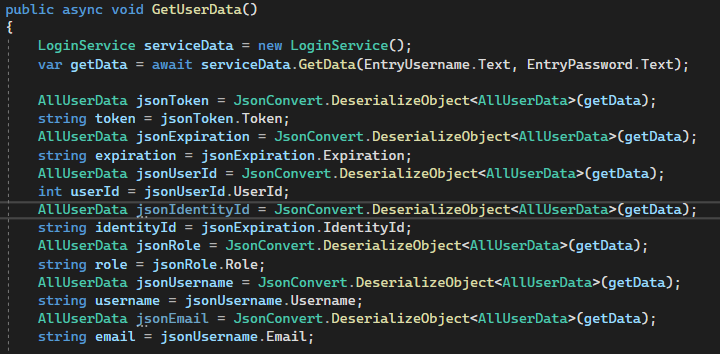
\includegraphics[width=10cm]{pics/Xamarin Frontend/4.png}
    \caption[Login]{UserData laden}
    \end{center}
\end{figure}
\newline
Nachdem die Logindaten erfolgreich geladen wurden, werden die Profildaten
wie Vorname, Nachname oder Schule mithilfe der userId geladen.
\newline
\begin{figure}[h]
    \begin{center}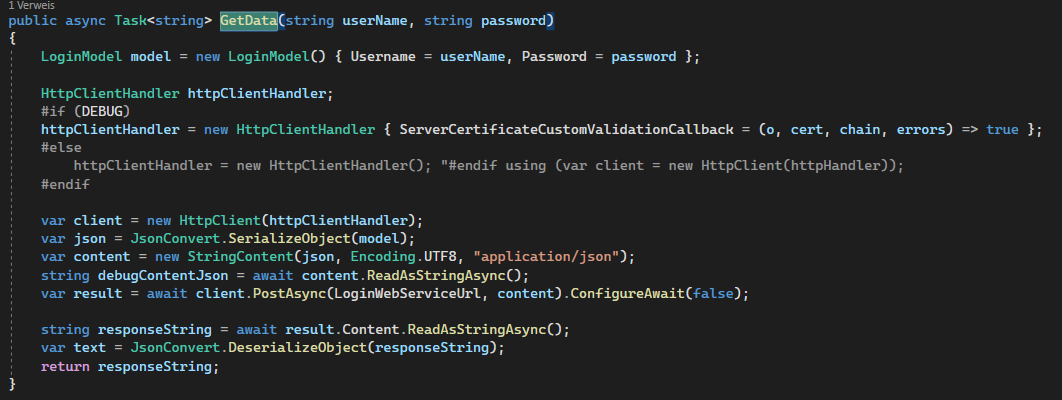
\includegraphics[width=10cm]{pics/Xamarin Frontend/5.png}
    \caption[Login]{UserData laden}
    \end{center}
\end{figure}
\newpage


\subsection{Registrierung}
Bei der Registrierung werden die eingegebenen Werte zunächst daraufhin überprüft, ob sie den Standards entsprechen. Danach wird registerService erstellt und Daten werden über restClient an RegisterModel übergeben. Feedback kann eine Bestätigung oder ein Fehler sein.
\begin{figure}[h]
    \begin{center}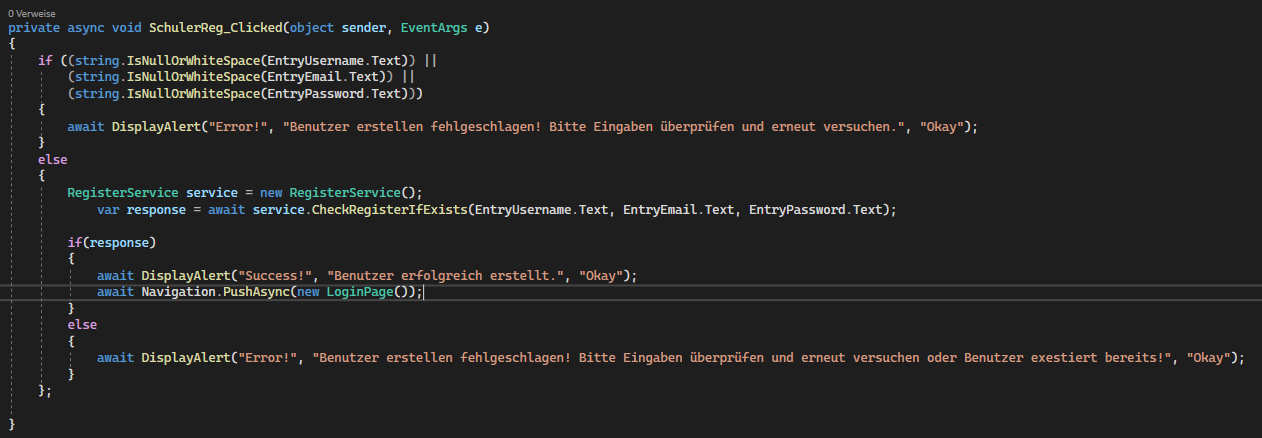
\includegraphics[width=10cm]{pics/Xamarin Frontend/6.png}
    \caption[Registrierung]{Konto erstellen}
    \end{center}
\end{figure}
\newline
Mit Hilfe von HttpClient werden die Daten im Backend geprüft und wir erhalten das Ergebnis.
\begin{figure}[h]
    \begin{center}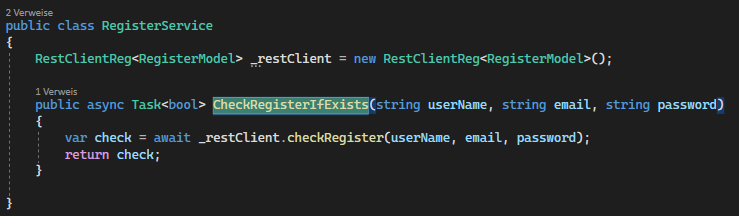
\includegraphics[width=10cm]{pics/Xamarin Frontend/7.png}
    \caption[Registrierung]{RestClient}
    \end{center}
\end{figure}
\newline
\begin{figure}[h]
    \begin{center}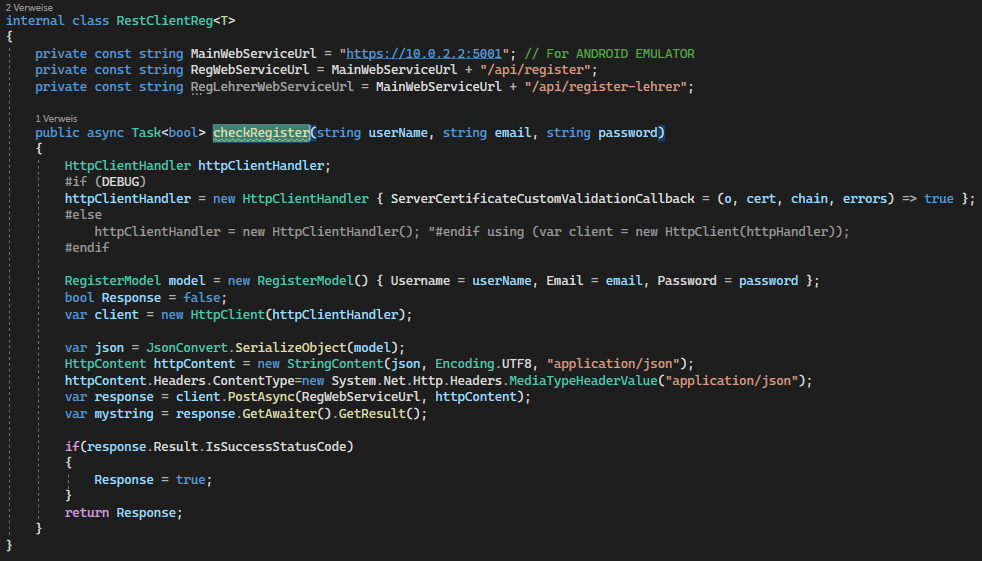
\includegraphics[width=10cm]{pics/Xamarin Frontend/8.png}
    \caption[Registrierung]{HttpClient}
    \end{center}
\end{figure}
\newpage

\subsection{Benutzerkontoverwaltung}
Bei der Anmeldung des Benutzers ruft die Methode sofort die Daten des Benutzers ab und sie werden auf der Kontoseite des Benutzers per Ansichtsliste angezeigt.
\begin{figure}[h]
    \begin{center}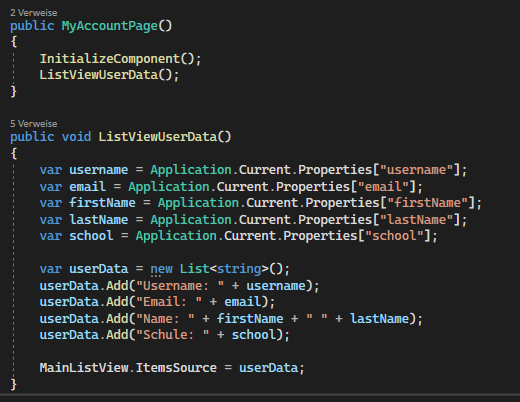
\includegraphics[width=10cm]{pics/Xamarin Frontend/9.png}
    \caption[MyAccount]{Benutzerkontoverwaltung Daten auslesen}
    \end{center}
\end{figure}
\newline
Wenn wir Daten wie E-Mail, Vorname, Nachname oder Schulname ändern möchten, tun wir dies über Tasks.
\begin{figure}[h]
    \begin{center}
    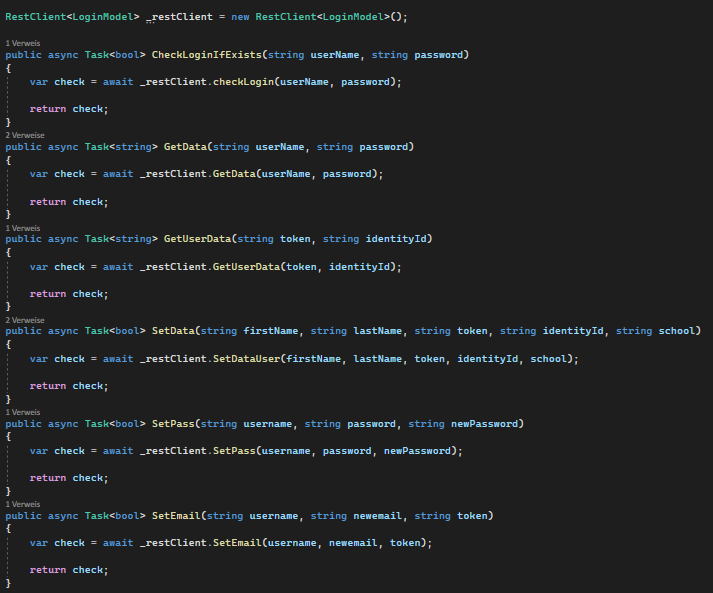
\includegraphics[width=6cm]{pics/Xamarin Frontend/tasks.png}\hfill
    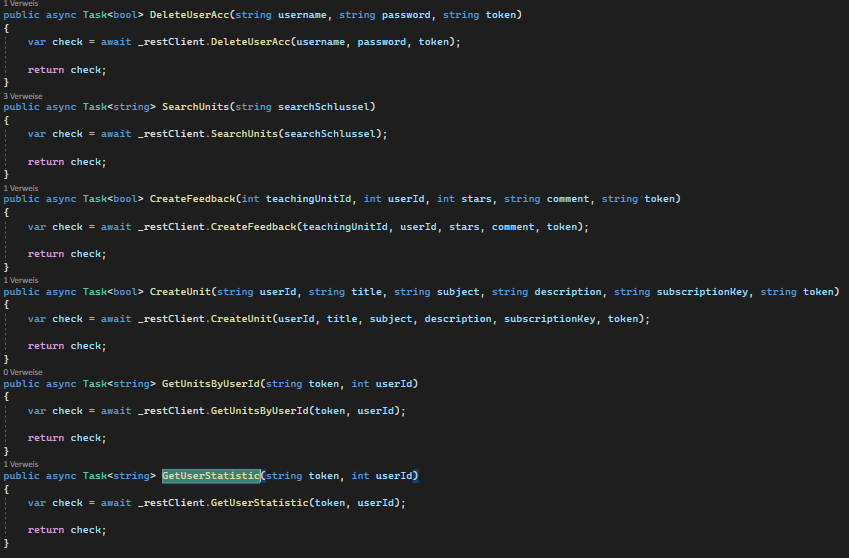
\includegraphics[width=6cm]{pics/Xamarin Frontend/tasks2.png}
    \caption[MyAccount]{Tasks}
    \end{center}
\end{figure}
\newline
Durch Drücken des Buttons Abmelden gelangen wir auf die Login-Homepage.
\begin{figure}[h]
    \begin{center}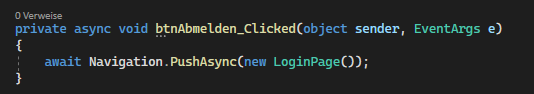
\includegraphics[width=10cm]{pics/Xamarin Frontend/abmelden.png}
    \caption[MyAccount]{Abmelden Button}
    \end{center}
\end{figure}
\newpage
Die Änderung der persönlichen Daten des Benutzers erfolgt auf die gleiche Weise. Die eingegebenen Daten werden an den LoginService gesendet und dann über den RestClient mit bool Tasks überprüft. Wenn die Antwort positiv ist, wurden die Daten geändert und gespeichert, andernfalls wird ein Fehler ausgegeben.
\newline
Nachfolgend finden Sie Beispiele für die Änderung von Daten wie E-Mail, Vorname, Nachname, E-Mail und Passwort.
\begin{figure}[h]
    \begin{center}
    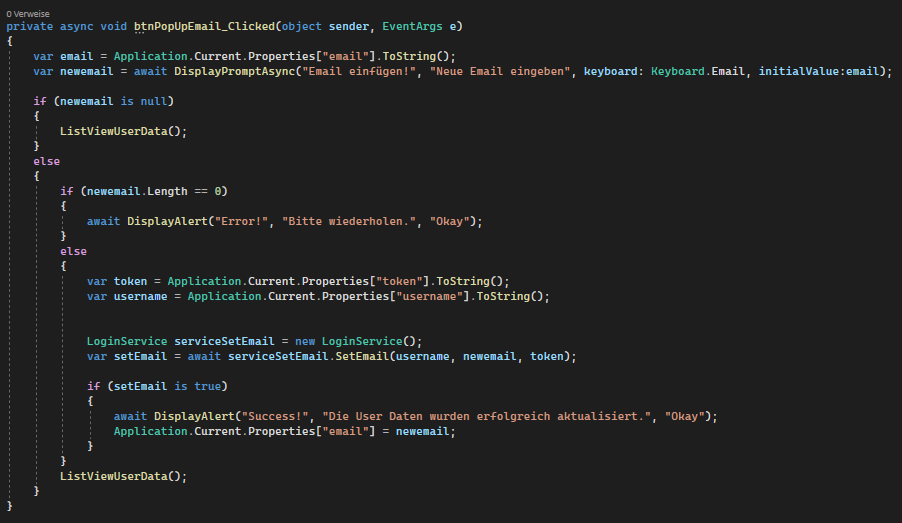
\includegraphics[width=6cm]{pics/Xamarin Frontend/email1.png}\hfill
    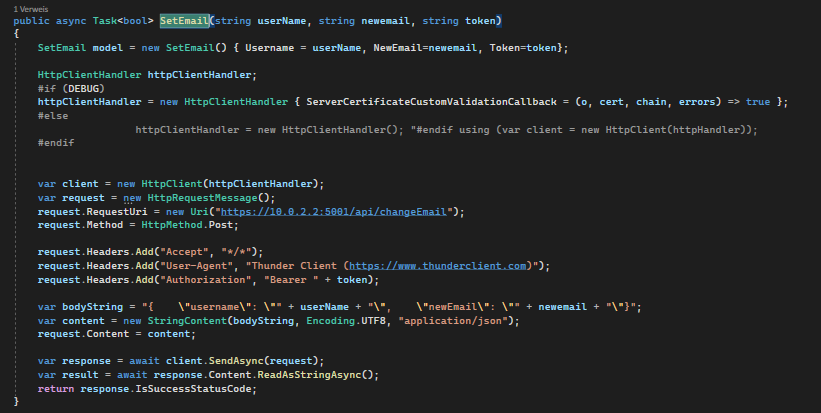
\includegraphics[width=6cm]{pics/Xamarin Frontend/email2.png}
    \caption[MyAccount]{Email ändern}
    \end{center}
\end{figure}
\begin{figure}[h]
    \begin{center}
    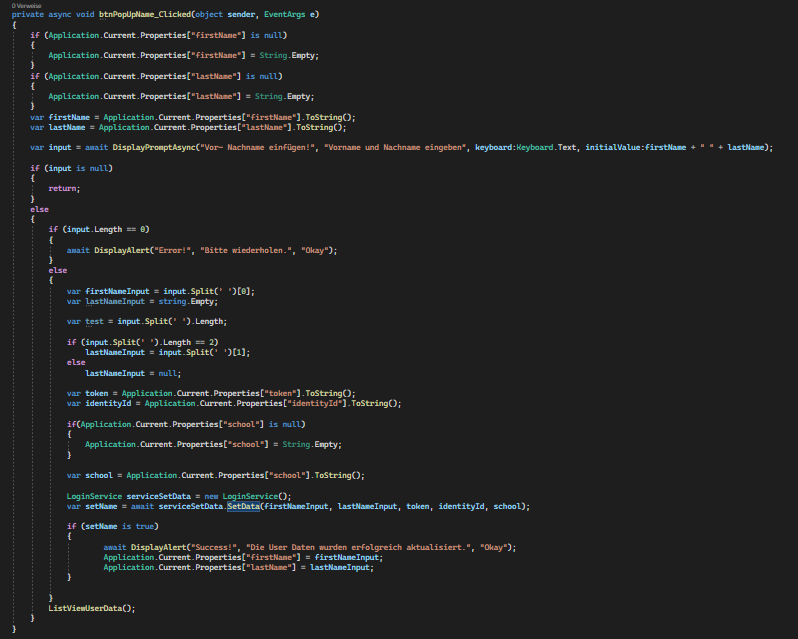
\includegraphics[width=6cm]{pics/Xamarin Frontend/name1.png}\hfill
    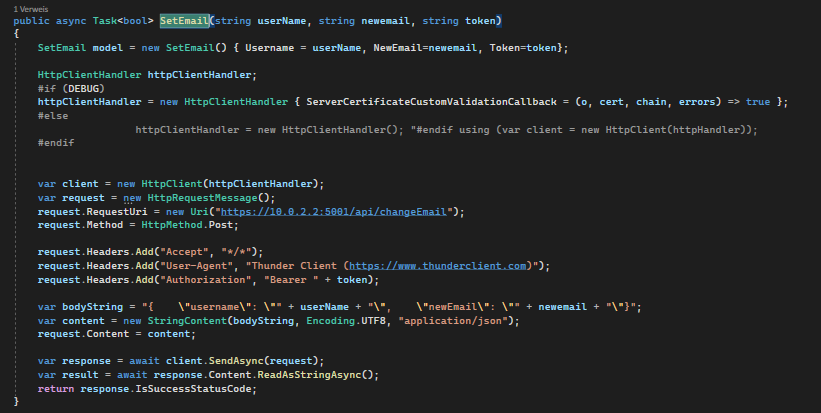
\includegraphics[width=6cm]{pics/Xamarin Frontend/email2.png}
    \caption[MyAccount]{Vorname und Nachname ändern}
    \end{center}
\end{figure}
\begin{figure}[h]
    \begin{center}
    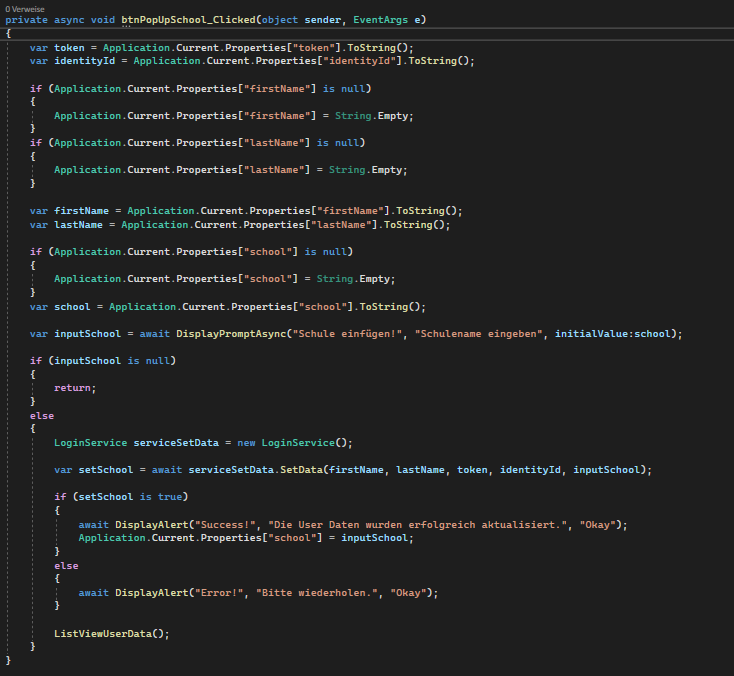
\includegraphics[width=6cm]{pics/Xamarin Frontend/school1.png}\hfill
    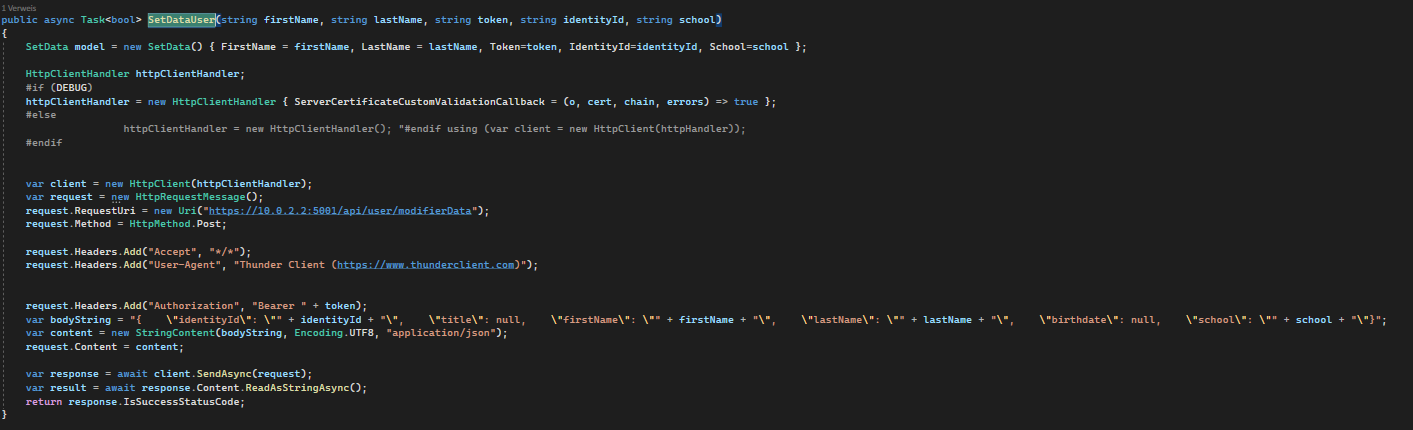
\includegraphics[width=6cm]{pics/Xamarin Frontend/school2.png}
    \caption[MyAccount]{Schule ändern}
    \end{center}
\end{figure}
\begin{figure}[h]
    \begin{center}
    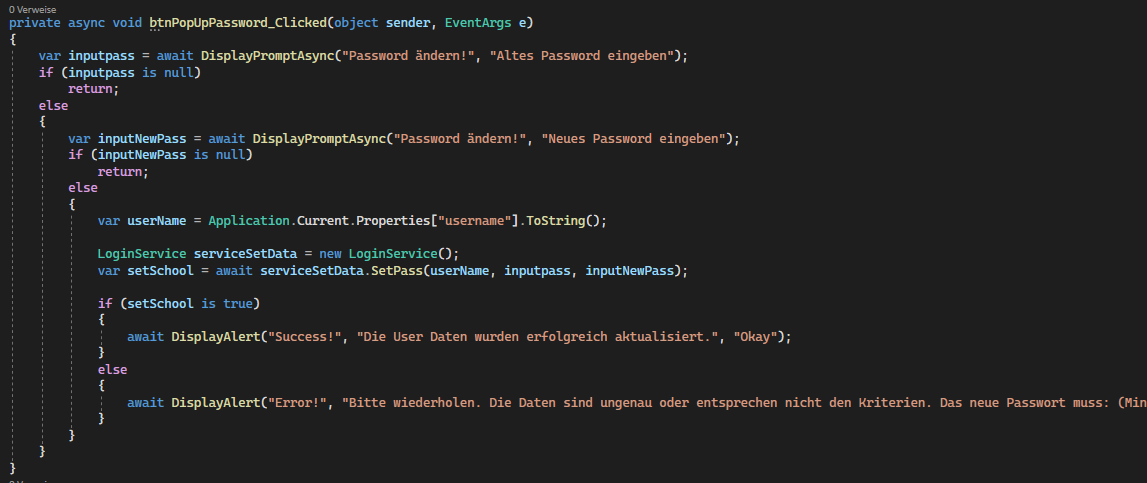
\includegraphics[width=6cm]{pics/Xamarin Frontend/pass1.png}\hfill
    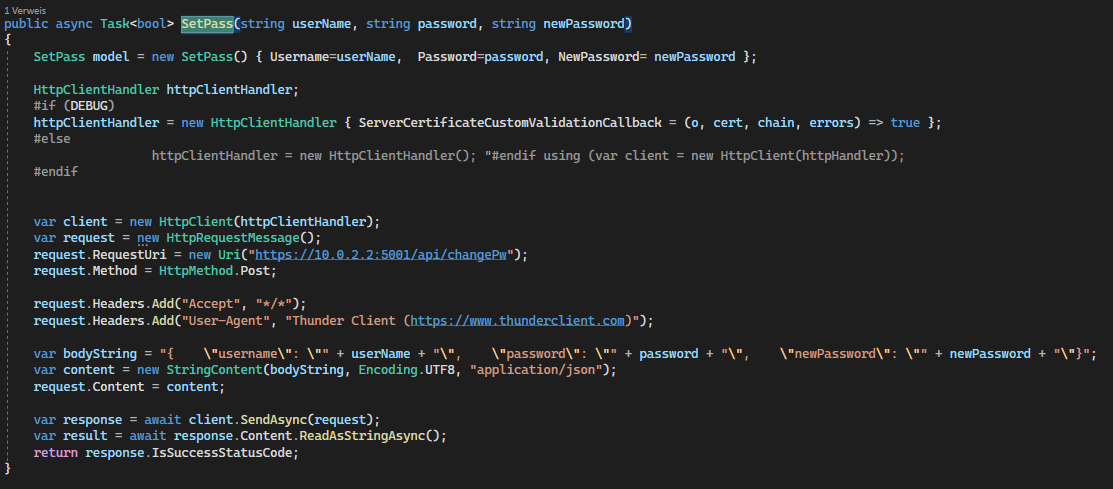
\includegraphics[width=6cm]{pics/Xamarin Frontend/pass2.png}
    \caption[MyAccount]{Password ändern}
    \end{center}
\end{figure}
\newline
Um ein Profil zu löschen, müssen Sie eine gültige E-Mail-Adresse eingeben. Dann werden die Daten an den LoginService gesendet und über RestClient prüfen wir, ob das Passwort korrekt ist. HttpClient sendet uns eine Antwort, und wenn dies zutrifft, werden die Daten und das Konto aus der Datenbank und dem Server gelöscht.
\begin{figure}[h]
    \begin{center}
    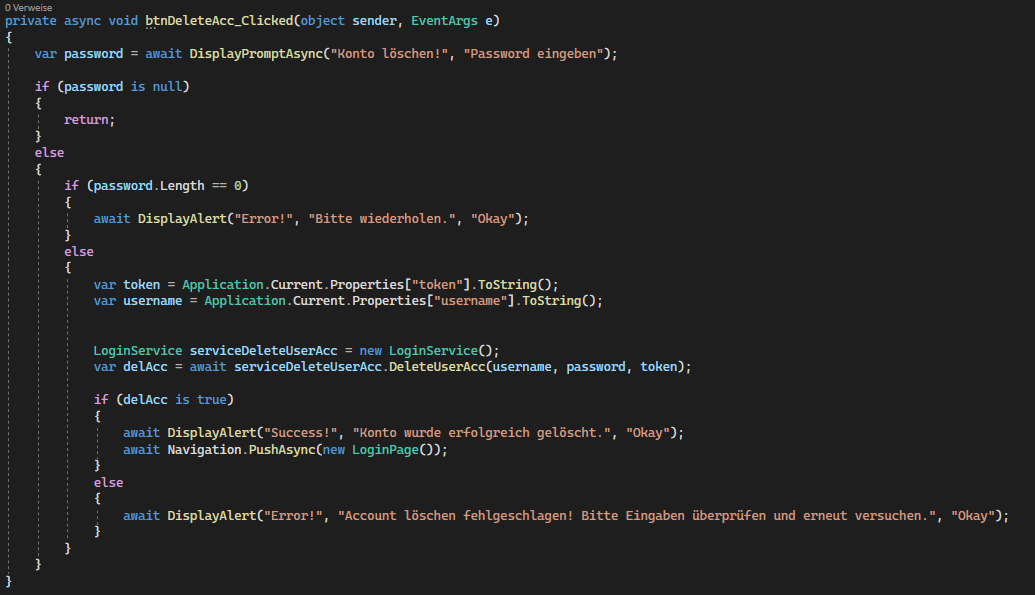
\includegraphics[width=6cm]{pics/Xamarin Frontend/accDelete.png}\hfill
    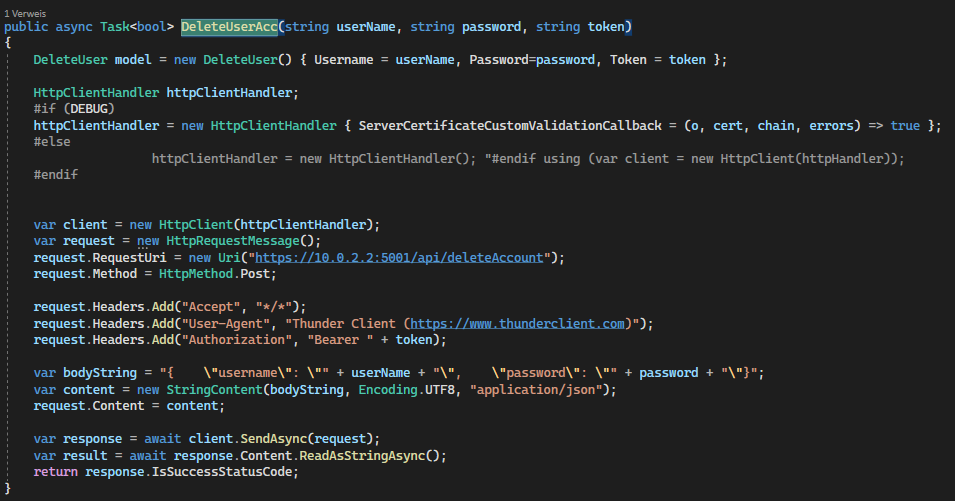
\includegraphics[width=6cm]{pics/Xamarin Frontend/accDelete2.png}
    \caption[MyAccount]{Konto löschen}
    \end{center}
\end{figure}
\newpage


\subsection{Statistik}
Beim Aufrufen der Statistikseite ziehen wir die Daten vom Server aus dem Backend.
Aus den gespeicherten Daten prüfen wir, ob es sich um einen Schüler oder einen Lehrer handelt, und rufen die korrekten Daten über LoginService und Statistics Task ab.
\begin{figure}[h]
    \begin{center}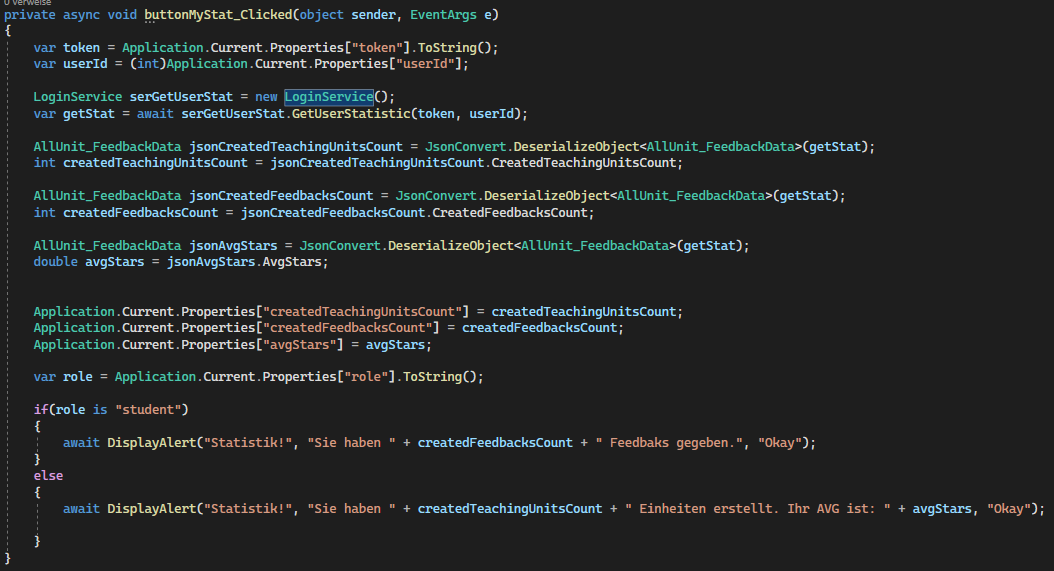
\includegraphics[width=10cm]{pics/Xamarin Frontend/statistic.png}
    \caption[Statistik]{Statistik Button}
    \end{center}
\end{figure}
\newline
Wir holen uns die Daten per httpclient vom Server und übertragen die Daten in den Response-String, damit wir ihn lesen können.
\begin{figure}[h]
    \begin{center}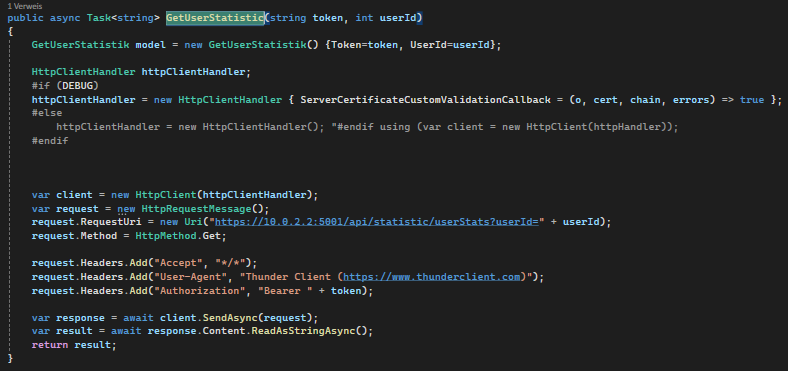
\includegraphics[width=10cm]{pics/Xamarin Frontend/stat http.png}
    \caption[Statistik]{HttpClient}
    \end{center}
\end{figure}
